% ~~~~~~~~~~~~~~~~~~~~~~~~~~~~~~~~~~~~~~~~~~~~~~~~~~~~~~~~~~~~~~~~~ %
\newif	\ifexternalize					%\externalizetrue			%
\newif	\ifshowonlynotes				%\showonlynotestrue			%
\newif	\ifhandout						%\handouttrue				%
\newif	\ifshowsolutions				%\showsolutionstrue			%
\newif	\ifshownotes					%\shownotestrue				%
%																	%
% enablers for conditional compiling through bash scripting			%
\ifdefined\EXTERNALIZE	\externalizetrue	\fi						%
\ifdefined\ONLYNOTES	\showonlynotestrue	\fi						%
\ifdefined\HANDOUT		\handouttrue		\fi						%
\ifdefined\SOLUTIONS	\showsolutionstrue	\fi						%
\ifdefined\NOTES		\shownotestrue		\fi						%
%																	%
% ~~~~~~~~~~~~ %
% tab size = 4 %
% ~~~~~~~~~~~~ %

% WARNING: if the compiler returns the error ``incompatible list can't be unboxed''
% try to decomment the following \RequirePackage command:
%\RequirePackage{atbegshi} 

\ifhandout
	\documentclass % ~~~~~~~~~~~~~~~~~~~~~~~~~~~~~~~~~~~~~~~~~~~~~~ %
	[																%
		11pt,														%
		professionalfont,											%
		hyperref={pdfpagelabels=false},								%
		xcolor	={dvipsnames, table},								%
		aspectratio	= 169,											%
		notheorems,													%
		handout,													%
	]																%
	{beamer}														%
	\usepackage{pgfpages}											%
	\ifshownotes													%
		\setbeameroption{show notes}								%
	\fi																%
	\ifshowonlynotes												%
		\setbeameroption{show only notes}							%
	\fi																%
	\pgfpagesuselayout{4 on 1}[a4paper,border shrink=5mm,landscape]	%
\else																%
	\documentclass % ~~~~~~~~~~~~~~~~~~~~~~~~~~~~~~~~~~~~~~~~~~~~~~ %
	[																%
		11pt,														%
		professionalfont,											%
		hyperref={pdfpagelabels=false},								%
		xcolor	={dvipsnames, table},								%
		aspectratio	= 169,											%
		notheorems,													%
	]																%
	{beamer}														%
	\usepackage{pgfpages}											%
	\ifshownotes													%
		\setbeameroption{show notes on second screen=left}			%
	\fi																%
	\ifshowonlynotes												%
		\setbeameroption{show only notes}							%
	\fi																%
\fi																	%
%																	%
% ~~~~~~~~~~~~~~~~~~~~~~~~~~~~~~~~~~~~~~~~~~~~~~~~~~~~~~~~~~~~~~~~~ %
%																	%
\usepackage{etex}													%
\usepackage[english]{babel}											%
\usepackage{type1cm}												%
\usepackage{type1ec}												%
\usepackage[T1]{fontenc}											%
\usepackage{lmodern}												%
\usepackage{amsmath,amssymb,amsfonts,amsthm}						%
\usepackage{graphicx}												%
\usepackage{hyperref}												%
\usepackage{booktabs}												%
\usepackage{bm}														%
\usepackage{dsfont}													%
\usepackage{array}													%
\usepackage{upquote}												%
\usepackage{acronym}												%
\usepackage{MnSymbol}												%
\usepackage[official]{eurosym}										%
\usepackage{xr}														%
\usepackage{varwidth}												%
\usepackage{tikz}													%
\usepackage[european]{circuitikz}									%
\usepackage{enumerate}												%
% \usepackage{enumitem}												%
\usetikzlibrary{shapes.geometric}									%
\usetikzlibrary{positioning}										%
\usetikzlibrary{calc}												%
\usetikzlibrary{matrix}												%
\usetikzlibrary{fit}												%
\usetikzlibrary{arrows.meta}										%
\usetikzlibrary{decorations.text}									%
\newcommand{\figurefilename}[1]{\ifexternalize \tikzsetnextfilename{#1} \fi}
\ifexternalize														%
	\usetikzlibrary{external}										%
	\tikzexternalize[shell escape=-enable-write18]					%
	\tikzset{external/force remake} 								%
\fi																	%
\usepackage{pgfplots}												%
\pgfplotsset{compat=1.14}											%
%																	%
% ~~~~~~~~~~~~~~~~~~~~~~~~~~~~~~~~~~~~~~~~~~~~~~~~~~~~~~~~~~~~~~~~~ %
%																	%
\def\DarkBlue		{black!40!blue}									%
\def\DarkGray		{black!70!white}								%
\def\DarkGreen		{black!40!green}								%
\def\DarkRed		{black!40!red}									%
\def\DarkYellow		{black!40!yellow}								%
\def\DarkOrange		{black!40!orange}								%
%																	%
\def\Blue			{black!10!blue}									%
\def\Gray			{black!50!white}								%
\def\Green			{black!10!green}								%
\def\Red			{black!10!red}									%
\def\Yellow			{black!10!yellow}								%
\def\Orange			{black!10!orange}								%
%																	%
\def\LightBlue		{white!40!blue}									%
\def\LightGray		{white!70!white}								%
\def\LightGreen		{white!40!green}								%
\def\LightRed		{white!40!red}									%
\def\LightYellow	{white!40!yellow}								%
\def\LightOrange	{white!40!orange}								%
%																	%
% ~~~~~~~~~~~~~~~~~~~~~~~~~~~~~~~~~~~~~~~~~~~~~~~~~~~~~~~~~~~~~~~~~ %
%																	%
\def\Background		{white}											%
\def\Foreground		{black}											%
\def\Primary		{Bittersweet!30!red}							%
\def\Secondary		{\Gray}											%
%																	%
\def\StrongPrimary	{\Primary!80!black}								%
\def\SoftPrimary	{\Primary!20!white}								%
\def\StrongSecondary{\Secondary!80!black}							%
\def\SoftSecondary	{\Secondary!20!white}							%
%																	%
% ~~~~~~~~~~~~~~~~~~~~~~~~~~~~~~~~~~~~~~~~~~~~~~~~~~~~~~~~~~~~~~~~~ %
%																	%
\graphicspath{{./Images/}}											%
\everymath{\displaystyle}											%
%																	%

\newcommand{\DefinedAs}			[0]	{\mathrel{\mathop:}=}
\newcommand{\IDefinedAs}		[0]	{=\mathrel{\mathop:}}


\newcommand{\ExponentialOf}		[1]	{\mathrm{exp} \left( #1 \right)}
\newcommand{\LogarithmOf}		[1]	{\mathrm{log} \left( #1 \right)}
\newcommand{\ConvexHullOf}		[1]	{\mathrm{c.h.} \left( #1 \right)}


\newcommand{\MaximumOfOne}		[1]	{\mathrm{max} \left\lbrace #1 \right\rbrace}
\newcommand{\MaximumOfTwo}		[2]	{\mathrm{max} \left\lbrace #1, #2 \right\rbrace)}
\newcommand{\MaximumOfThree}	[3]	{\mathrm{max} \left\lbrace #1, #2, #3 \right\rbrace)}
\newcommand{\MinimumOfOne}		[1]	{\mathrm{min} \left\lbrace #1 \right\rbrace}
\newcommand{\MinimumOfTwo}		[2]	{\mathrm{min} \left\lbrace #1, #2 \right\rbrace)}
\newcommand{\MinimumOfThree}	[3]	{\mathrm{min} \left\lbrace #1, #2, #3 \right\rbrace)}


\newcommand{\CostFunction}				[0]	{Q}
\newcommand{\CostFunctionOf}			[1]	{\CostFunction \left( #1 \right)}
\newcommand{\CostFunctionOfSensor}		[1]	{\CostFunction_{#1}}
\newcommand{\CostFunctionOfSensorOf}	[2]	{\CostFunctionOfSensor{#1} \left( #2 \right)}


\newcommand{\KroneckerDeltaOf}			[2]	{\delta_{#1 #2}}


\newcommand{\FloorOf}			[1]	{\lfloor #1 \rfloor}
\newcommand{\CeilOf}			[1]	{\lceil #1 \rceil}


\newcommand{\GammaFunctionOf}	[1]	{\Gamma \left( #1 \right)}

\newcommand{\IdentityMatrix}		[1]	{I_{#1}}
\newcommand{\OnesVector}			[1]	{\mathds{1}_{#1}}

\newcommand{\TraceOf}				[1]	{\text{tr} \left( #1 \right)}
\newcommand{\DeterminantOf}			[1]	{\text{det} \left( #1 \right)}
\newcommand{\SetOfEigenvaluesOf}	[1]	{\text{eig} \left( #1 \right)}

\newcommand{\Eigenvalue}			[1]	{\lambda_{#1}}
\newcommand{\Eigenvector}			[1]	{v_{#1}}
\newcommand{\MaximalEigenvalue}		[0]	{\lambda_{\text{max}}}
\newcommand{\MinimalEigenvalue}		[0]	{\lambda_{\text{min}}}

\newcommand{\SpectralRadius}		[0]	{\mu}
\newcommand{\SpectralRadiusOf}		[1]	{\SpectralRadius \left( #1 \right)}


\newcommand{\GaussianDistribution}					[2]	{\mathcal{N} \left( #1, #2 \right)}
\newcommand{\GammaDistribution}						[2]	{\text{Gamma} \left( #1, #2 \right)}
\newcommand{\ChiSquareDistribution}					[0]	{\chi^{2}}
\newcommand{\ChiSquareDistributionOfIndex}			[1]	{\ChiSquareDistribution \left( #1 \right)}
\newcommand{\InverseChiSquareDistribution}			[0]	{\text{Inv-}\chi^{2}}
\newcommand{\InverseChiSquareDistributionOfIndex}	[1]	{\InverseChiSquareDistribution \left( #1 \right)}
\newcommand{\UniformDistribution}					[2]	{\mathcal{U} \left[ #1, #2 \right]}
\newcommand{\ExponentialDistribution}				[1]	{\text{Exp} \left( #1 \right)}


\newcommand{\Reals}						[0]	{\mathbb{R}}
\newcommand{\PositiveReals}				[0]	{\mathbb{R}_{+}}
\newcommand{\Naturals}					[0]	{\mathbb{N}}
\newcommand{\PositiveNaturals}			[0]	{\mathbb{N}_{+}}

\newcommand{\SetOfSquareSummableInfiniteVectors}			[0]	{\ell}
\newcommand{\SetOfWeightedSquareSummableInfiniteVectors}	[0]	{\textsl{l}_{\RKHS}}
\newcommand{\SetOfSquareIntegrableFunctions}				[0]	{\textsl{L}^{2}}
\newcommand{\SetOfSquareIntegrableFunctionsIn}				[1]	{\textsl{L}^{2} \left( #1 \right)}

\newcommand{\Probability}			[0]	{\mathbb{P}}
\newcommand{\ProbabilityOf}			[1]	{\Probability \left[ #1 \right]}
\newcommand{\ProbabilityOfGiven}	[2]	{\ProbabilityOf{ #1 \; \left| \; #2 \right.}}


\newcommand{\ProbabilityDistribution}		[0]	{P}
\newcommand{\ProbabilityDistributionOf}		[1]	{\ProbabilityDistribution \left( #1 \right)}
\newcommand{\ProbabilityDistributionOfGiven}[2]	{\ProbabilityDistributionOf{ #1 \left| #2 \right. }}
%
\newcommand{\ProbabilityDistributionOfRV}	[1]	{\ProbabilityDistribution_{#1}}
\newcommand{\ProbabilityDistributionOfRVOf}	[2]	{\ProbabilityDistributionOfRV{#1} \left( #2 \right)}
\newcommand{\ProbabilityDistributionOfRVOfGiven}	[3]
		   {\ProbabilityDistributionOfRVOf{#1}{ #2 \left| #3 \right. }}


\newcommand{\ProbabilityDensity}			[0]	{p}
\newcommand{\ProbabilityDensityOf}			[1]	{\ProbabilityDensity \left( #1 \right)}
\newcommand{\ProbabilityDensityOfGiven}		[2]	{\ProbabilityDensityOf{ #1 \left| #2 \right. }}
%
\newcommand{\ProbabilityDensityOfRV}		[1]	{\ProbabilityDensity_{#1}}
\newcommand{\ProbabilityDensityOfRVOf}		[2]	{\ProbabilityDensityOfRV{#1} \left( #2 \right)}
\newcommand{\ProbabilityDensityOfRVOfGiven}	[3] {\ProbabilityDensityOfRVOf{#1}{ #2 \left| #3 \right. }}


\newcommand{\ProbabilityMassFunction}		[0]	{m}
\newcommand{\ProbabilityMassFunctionOf}		[1]	{\ProbabilityMassFunction \left( #1 \right)}
\newcommand{\ProbabilityMassFunctionOfGiven}[2]	{\ProbabilityMassFunctionOf{ #1 \left| #2 \right. }}
%
\newcommand{\ProbabilityMassFunctionOfRV}	[1]	{\ProbabilityMassFunction_{#1}}
\newcommand{\ProbabilityMassFunctionOfRVOf}	[2]	{\ProbabilityMassFunctionOfRV{#1} \left( #2 \right)}
\newcommand{\ProbabilityMassFunctionOfRVOfGiven}		[3]
		   {\ProbabilityMassFunctionOfRVOf{#1}{ #2 \left| #3 \right. }}


\newcommand{\Expectation}					[0]	{\mathbb{E}}
\newcommand{\ExpectationOf}					[1]	{\Expectation \left[ #1 \right]}
\newcommand{\ExpectationOfOnMeasure}		[2]	{\Expectation_{#2} \left[ #1 \right]}
\newcommand{\ExpectationOfGiven}			[2]	{\ExpectationOf{ #1 \; \left| \; #2 \right. }}
\newcommand{\ExpectationOfOnMeasureGiven}	[3]	{\ExpectationOfOnMeasure{#1 \; \left| \; #3 \right.}{#2}}


\newcommand{\Variance}				[0]	{\mathrm{var}}
\newcommand{\VarianceOf}			[1]	{\Variance \left( #1 \right)}
\newcommand{\VarianceOfGiven}		[2]	{\VarianceOf{ #1 \; \left| \; #2 \right. }}


\newcommand{\Covariance}			[0]	{\mathrm{cov}}
\newcommand{\CovarianceOf}			[2]	{\Covariance \left( #1, #2 \right)}
\newcommand{\CovarianceOfGiven}		[3]	{\Covariance \left( #1, #2 \; \left| \; #3 \right. \right)}


\newcommand{\BayesEstimatorOfGiven}	[2]	{\widehat{\Expectation} \left[ #1 \; \left| \; #2 \right. \right] }


\newcommand{\IndicatorFunctionOf}	[1]	{\mathds{1} \left\lbrace #1 \right\rbrace}


\newcommand{\SufficientStatistic}	[0]	{T}
\newcommand{\SufficientStatisticOf}	[1]	{\SufficientStatistic \left( #1 \right)}

\newcommand{\Fingers}
{
	\begin{itemize}
		\item yes \hfill (1 finger)
		\item yes, maybe \hfill (2 fingers)
		\item I don't know \hfill (3 fingers)
		\item no, maybe not \hfill (4 fingers)
		\item no \hfill (5 fingers)
	\end{itemize}
}

\newcommand	{\SuchThat}				{s.t.\ }

\newcommand	{\Section}				[0]	{Sec.}
\newcommand	{\Sections}				[0]	{Secc.}
\newcommand	{\Equation}				[0]	{Equ.}
\newcommand	{\Equations}			[0]	{Equu.}
\newcommand	{\Figure}				[0]	{Fig.}
\newcommand	{\Figures}				[0]	{Figg.}
\newcommand	{\Table}				[0]	{Tab.}
\newcommand	{\Tables}				[0]	{Tabb.}
\newcommand	{\Algorithm}			[0]	{Alg.}
\newcommand	{\Algorithms}			[0]	{Algg.}
\newcommand	{\Proposition}			[0]	{Prop.}
\newcommand	{\Propositions}			[0]	{Propp.}
\newcommand	{\Hypothesis}			[0]	{Hyp.}
\newcommand	{\Hypotheses}			[0]	{Hypp.}

\setbeamertemplate{theorems}[numbered]
\newtheorem{question}{Question}

\newcounter{QuestionsCounter}
\stepcounter{QuestionsCounter}

\newcommand	{\QuestionID}		[1]	{\JustSecondary{(ID: #1)} \label{question:#1} \stepcounter{QuestionsCounter}}
\newcommand	{\QuestionKCs}		[1] {}
\newcommand	{\QuestionKCsTaxonomies}	[1] {}
\newcommand	{\QuestionNotes}	[1] {}
\newcommand	{\QuestionBody}		[1] {#1}
\newcommand	{\QuestionImage}	[2] {\begin{center} \includegraphics[#1]{#2} \end{center}}
\newcommand	{\QuestionAnswers}	[1] {\begin{enumerate} #1 \end{enumerate}}
\newcommand	{\QuestionSolution}	[1] {\ifshowsolutions \note<1->{#1} \fi}
\newcommand	{\QuestionAuthor}	[1] {}
\newcommand	{\QuestionVersion}	[1] {}







\newcommand{\answer}		[0]
{
	\item[\addtocounter{enumi}{1} \tikz{ \node [anchor = base, baseline, minimum width = 0.6cm, minimum height = 0.6cm, draw] {\arabic{enumi}};}]
}

\newcommand{\correctanswer}	[0]
{
	\ifshowsolutions
		\item[\addtocounter{enumi}{1} \tikz{ \node [anchor = base, baseline, minimum width = 0.6cm, minimum height = 0.6cm, draw, fill = red!30!white] {\arabic{enumi}};}]
	\else
		\answer
	\fi
}

% \newcommand{\hideableanswer}[1]{\item \ifshowsolutions #1 \fi}





\pgfdeclarelayer{ultrabackground}
\pgfdeclarelayer{background}
\pgfdeclarelayer{foreground}
\pgfsetlayers{ultrabackground,background,main,foreground}
% \begin{pgfonlayer}{background} 
% \end{pgfonlayer}


\newcommand{\JustPrimary}		[1]{\textcolor{\StrongPrimary}{#1}}
\newcommand{\ItPrimary}			[1]{\textcolor{\StrongPrimary}{\textit{#1}}}
\newcommand{\BoldPrimary}		[1]{\textcolor{\StrongPrimary}{\textbf{#1}}}
\newcommand{\BoldItPrimary}		[1]{\textcolor{\StrongPrimary}{\textit{ \textbf{#1} }}}
\newcommand{\ItBoldPrimary}		[1]{\BoldItPrimary{#1}}
\newcommand{\MathBoxPrimary}	[1]{\colorbox{\SoftPrimary}{#1}}
%
\newcommand{\JustSecondary}		[1]{\textcolor{\StrongSecondary}{#1}}
\newcommand{\ItSecondary}		[1]{\textcolor{\StrongSecondary}{\textit{#1}}}
\newcommand{\BoldSecondary}		[1]{\textcolor{\StrongSecondary}{\textbf{#1}}}
\newcommand{\BoldItSecondary}	[1]{\textcolor{\StrongSecondary}{\textit{ \textbf{#1} }}}
\newcommand{\ItBoldSecondary}	[1]{\BoldItSecondary{#1}}
\newcommand{\MathBoxSecondary}	[1]{\colorbox{\SoftSecondary}{#1}}
%
\newcommand{\Code}				[1]{\texttt{\textcolor{\StrongSecondary}{#1}}}


\newcommand{\NewSection}		[1]
{
	\subsection{#1}
	\label{sec: #1}
	\setbeamercolor{background canvas}{bg=\SoftPrimary}
	\begin{frame}
		\begin{center}
			\Large #1
		\end{center}
		\note<1-1>{\begin{itemize}
			\item 
		\end{itemize}}
	\end{frame}
	\setbeamercolor{background canvas}{bg=white}
}

\newcommand{\QuestionMark}		[0]
{
	\setbeamercolor{background canvas}{bg=\SoftSecondary}
	\begin{frame}
		\begin{center}
			\Large ?
		\end{center}
		\note<1-1>{\begin{itemize}
			\item 
		\end{itemize}}
	\end{frame}
	\setbeamercolor{background canvas}{bg=white}
}

\newcommand {\PrimaryRectangle} [1]
{
	\begin{center}
	\begin{tikzpicture}
		%
		\node
		[
			shape			= rectangle,		% shape
			rounded corners	= 0.2cm,			% shape
			minimum width	= 0.7cm,			%
			minimum height	= 0.7cm,			%
			line width		= 0cm,				% thickness of the border
			fill			= \SoftPrimary,		%
			draw			= \StrongPrimary,	% draw the border with this color
			line width		= 0.1cm,			% thickness
			text width		= 0.8\textwidth,	% max. width of the text
			align			= center,			% text alignment
			inner xsep		= 0.2cm,			%
			inner ysep		= 0.2cm,			%
		]
		{#1};
		%
	\end{tikzpicture}
	\end{center}
}

\newcommand {\SecondaryRectangle} [1]
{
	\begin{center}
	\begin{tikzpicture}
		%
		\node
		[
			shape			= rectangle,		% shape
			rounded corners	= 0.2cm,			% shape
			minimum width	= 0.7cm,			%
			minimum height	= 0.7cm,			%
			line width		= 0cm,				% thickness of the border
			fill			= \SoftSecondary,	%
			draw			= \StrongSecondary,	% draw the border with this color
			line width		= 0.1cm,			% thickness
			text width		= 0.9\textwidth,	% max. width of the text
			align			= center,			% text alignment
			inner xsep		= 0.2cm,			%
			inner ysep		= 0.2cm,			%
		]
		{#1};
		%
	\end{tikzpicture}
	\end{center}
}

\newcommand {\PrimaryRectangleWithCaption} [3]
{
	\begin{center}
	\begin{tikzpicture}
		%
		\node (a)
		[
			shape			= rectangle,		% shape
			rounded corners	= 0.2cm,			% shape
			minimum width	= 0.7cm,			%
			minimum height	= 0.7cm,			%
			fill			= \SoftPrimary,		%
			draw			= \StrongPrimary,	% draw the border with this color
			line width		= 0.1cm,			% thickness
			text width		= 0.8\textwidth,	% max. width of the text
			align			= center,			% text alignment
			inner xsep		= 0.3cm,			%
			inner ysep		= 0.3cm,			%
		]
		{#2};
		%
		\node
		[
			shape			= rectangle,		% shape
			rounded corners	= 0.2cm,			% shape
			anchor			= mid,
			fill			= \SoftPrimary,		%
			draw			= \StrongPrimary,	% draw the border with this color
			text			= \StrongPrimary,	%
			align			= center,			% text alignment
			line width		= 0.1cm,			% thickness
			inner xsep		= 0.2cm,			%
			inner ysep		= 0.2cm,			%
		]
		at (a.#3)
		{#1};
		%
	\end{tikzpicture}
	\end{center}
}

\newcommand {\SecondaryRectangleWithCaption} [3]
{
	\begin{center}
	\begin{tikzpicture}
		%
		\node (a)
		[
			shape			= rectangle,		% shape
			rounded corners	= 0.2cm,			% shape
			minimum width	= 0.7cm,			%
			minimum height	= 0.7cm,			%
			fill			= \SoftSecondary,	%
			draw			= \StrongSecondary,	% draw the border with this color
			line width		= 0.1cm,			% thickness
			text width		= 0.8\textwidth,	% max. width of the text
			align			= center,			% text alignment
			inner xsep		= 0.3cm,			%
			inner ysep		= 0.3cm,			%
		]
		{#2};
		%
		\node
		[
			shape			= rectangle,		% shape
			rounded corners	= 0.2cm,			% shape
			anchor			= mid,
			fill			= \SoftSecondary,	%
			draw			= \StrongSecondary,	% draw the border with this color
			text			= \StrongSecondary,	%
			align			= center,			% text alignment
			line width		= 0.1cm,			% thickness
			inner xsep		= 0.2cm,			%
			inner ysep		= 0.2cm,			%
		]
		at (a.#3)
		{#1};
		%
	\end{tikzpicture}
	\end{center}
}

\newcommand{\InsertImage}[3] % path / height / width
{
	\begin{tikzpicture}[remember picture, overlay]
	\node
	[
		shape			= rectangle,		% shape
		minimum height	= #2cm,				% | minimum size of the node
		minimum width	= #3cm,				% |
 		path picture	=
		{\node at (path picture bounding box.center)
		{\includegraphics[height = #2cm, width = #3cm]
		{#1}};}
	]{};
	\end{tikzpicture}
}

\newcommand{\InsertImageAt}[5] % path / height / width / xshift / yshift
{
	\begin{tikzpicture}[remember picture, overlay]
	\node
	[
		shape			= rectangle,		% shape
		minimum height	= #2cm,				% | minimum size of the node
		minimum width	= #3cm,				% |
		xshift 			= #4cm,
		yshift			= #5cm,
 		path picture	=
		{\node at (path picture bounding box.center)
		{\includegraphics[height = #2cm, width = #3cm]
		{#1}};}
	]
	at (current page.center)
	{};
	\end{tikzpicture}
}

\newcommand{\InsertTextAt}[3] % text / xshift / yshift
{
	\begin{tikzpicture}[remember picture, overlay]
	\node
	[
		shape			= rectangle,		% shape
		xshift 			= #2cm,
		yshift			= #3cm,
	]
	at (current page.center)
	{#1};
	\end{tikzpicture}
}

\newcommand{\Formula}[2]
{
	\begin{frame}[t]
	\ifexternalize
		\tikzsetnextfilename{formula-#1}
	\fi
	\begin{tikzpicture}
		\node
		{$
			#2
		$};
	\end{tikzpicture}
	\end{frame}
}

										%
\pgfdeclarelayer{ultrabackground}
\pgfdeclarelayer{background}
\pgfdeclarelayer{foreground}
\pgfsetlayers{ultrabackground,background,main,foreground}

\tikzset
{
	FancyCircle/.style =
	{
		shape					= circle,
		line width				= 0.1cm,
		align					= center,
		inner xsep				= 0.1cm,
		inner ysep				= 0.1cm,
		text width				= 2.4cm,
%		circular drop shadow	= { shadow scale = 1.05 },
		minimum size			= 0.5cm,
		fill					= \SoftSecondary,
		draw					= \StrongPrimary,
	},
	NormalNodeStyle/.style =
	{
		circle,									% shape
		minimum size	= 0.25cm,				%
		rotate			= 0,					% angle of rotation
		scale			= 1.0,					% scaling factor
		thick,									% thickness of the border
		fill			= \LightGray,			% monocolored
		text			= black,				% colour of the fonts
		draw			= black,				% colour of the border
		font			= \scriptsize,			%
		text centered,							% text alignment 
		inner xsep		= 0mm,					%
		inner ysep		= 0mm					%
	},
	NormalEdgeStyle/.style = 
	{
		dash pattern	= on .05cm off .02cm,
		line width		= 0.03cm,
		color 			= \DarkGray,
		shorten	<		= 0.05cm,
		shorten	>		= 0.05cm,
	},
	AlertedNodeStyle/.style =
	{
		NormalNodeStyle,						% shape
		fill			= \SoftPrimary,			% monocolored
		draw			= \StrongPrimary,		% colour of the border
	},
	SecondaryRectangleStyle/.style =
	{
		shape			= rectangle,		% shape
		rounded corners	= 0.2cm,			% shape
		minimum width	= 0.7cm,			%
		minimum height	= 0.7cm,			%
		line width		= 0cm,				% thickness of the border
		fill			= \SoftSecondary,		%
		draw			= \SoftSecondary,		% draw the border with this color
		line width		= 0.1cm,			% thickness
%		text width		= 0.8\textwidth,	% max. width of the text
		align			= center,			% text alignment
		inner xsep		= 0.2cm,			%
		inner ysep		= 0.2cm,			%
	},
	PrimaryRectangleStyle/.style =
	{
		SecondaryRectangle,
		fill			= white,
		draw			= \StrongPrimary,
	},
	SecondaryArrowStyle/.style =
	{
		line width		= 0.05cm,
		color			= \SoftSecondary,
		shorten <		= 0.1cm,
		shorten >		= 0.1cm,
		-latex
	},
	PrimaryArrowStyle/.style =
	{
		SecondaryArrow,
		color			= \SoftPrimary,
	},
	-|-/.style =
	{
		to path =
		{
			(\tikztostart) -| ($(\tikztostart)!#1!(\tikztotarget)$) |- (\tikztotarget)
			\tikztonodes
		}
	},
	-|-/.default = 0.5,
	|-|/.style =
	{
		to path =
		{
			(\tikztostart) |- ($(\tikztostart)!#1!(\tikztotarget)$) -| (\tikztotarget)
			\tikztonodes
		}
	},
	|-|/.default = 0.5,
}

% 
% \pgfplotsset
% {
% 	every axis/.append style = 
% 	{
% 		anchor					= north,
% 		width					= 0.7\columnwidth,
% 		height					= 0.5\columnwidth,
% 		axis x line				= center,
% 		axis y line				= left,
% 		xlabel near ticks,
% 		xmin					= 0,
% 		xmax					= 9.5,
% 		cycle list name			= mycyclelist,
% 		ymin					= -0.5,
% 		ymax					= 1.2,
% 		xtick					= {\empty},
% 		ytick					= {0},
% 		legend pos				= outer north east,
% 		legend style			=
% 		{
% 			draw				= none,
% 			fill				= none,
% 		},
% 		legend cell align		= left, % left | center | right
% 		title style				= {text width = 0.9\columnwidth, align = center, draw, rounded corners, fill = white!95!black},
% 	}
% }
% 
							%
% ~~~~~~~~~~~~~~~~~~~~~~~~~~~~~~~~~~~~~~~~~~~~~~~~~~~~~~~~~~~~~~~~~~~~~~~~~~~~~~~~~~~~~ %
%																						%
\usetheme			[]							{default}								%
\usefonttheme		[]							{default}								%
\usecolortheme		[]							{default}								%
\useinnertheme		[shadow]					{rounded}								%
\useoutertheme		[]							{default}								%
%																						%
\setbeamercolor		{normal text}				{bg=\SoftSecondary,	fg=\StrongPrimary}	%
\setbeamercolor		{structure}					{bg=\SoftSecondary,	fg=\StrongPrimary}	%
%																						%
\setbeamercolor		{frametitle}				{bg=, fg=\StrongPrimary}				%
\setbeamercolor		{block title}				{bg=\SoftSecondary,	fg=\StrongPrimary}	%
\setbeamercolor		{block title alerted}		{bg=\SoftSecondary,	fg=\StrongPrimary}	%
\setbeamercolor		{block title example}		{bg=\SoftSecondary,	fg=\StrongPrimary}	%
\setbeamercolor		{block body}				{bg=\Background,	fg=\Foreground}		%
\setbeamercolor		{block body alerted}		{bg=\Background,	fg=\Foreground}		%
\setbeamercolor		{block body example}		{bg=\Background,	fg=\Foreground}		%
%																						%
\setbeamercolor		{alerted text}				{bg=\Background,	fg=\StrongPrimary}	%
\setbeamercolor		{section in toc}			{bg=\Background,	fg=\Foreground}		%
\setbeamercolor		{math text}					{bg=\Background,	fg=\Foreground}		%
\setbeamercolor		{math text inlined}			{bg=\Background,	fg=\Foreground}		%
\setbeamercolor		{math text displayed}		{bg=\Background,	fg=\Foreground}		%
\setbeamercolor		{normal text}				{bg=\Background,	fg=\Foreground}		%
\setbeamercolor		{normal text in math text}	{bg=\Background,	fg=\Foreground}		%
%																						%
\setbeamercolor		{item}						{use={structure,normal text}}			%
\setbeamercolor		{background canvas}			{bg=\Background}						%
\setbeamertemplate	{navigation symbols}		{}										%
\setbeamercovered	{transparent=0}														%
\setbeamersize		{description width of={a}}											%
%																						%
% ~~~~~~~~~~~~~~~~~~~~~~~~~~~~~~~~~~~~~~~~~~~~~~~~~~~~~~~~~~~~~~~~~~~~~~~~~~~~~~~~~~~~~ %

\everymath={\displaystyle}

% \useinnertheme	[]{default}
% \useinnertheme	[]{circles}
% \useinnertheme	[]{rectangles}
% \useinnertheme	[]{rounded}
% \useinnertheme	[shadow]{rounded}
% \useinnertheme	[]{inmargin}


% -------------------------------------------------------------------------
% Logo settings
%\logo{\includegraphics[height = 1cm]{logo}}


% -------------------------------------------------------------------------
% if you DO want the navigation symbols you have to comment the following line
\setbeamertemplate{navigation symbols}{}


% -------------------------------------------------------------------------
% slides number
\setbeamertemplate{footline}{\hfill \insertframenumber \vspace{0.1cm} \hspace{0.1cm}} 


% -------------------------------------------------------------------------
% settings of the text to be unshown. Options:
% -> invisible	[text is invisible until it must appear]
% -> trasparent	[text is opaque (in %) until it must appear]
% -> dynamic	[text appears dynamically: initially invisible, then opaque and then appears fully]
\setbeamercovered{transparent=0}


% -------------------------------------------------------------------------
% if the frame is not fully occupied by text put the white space on the bottom
\raggedbottom


\providecommand\thispdfpagelabel[1]{}			% TEMPORARY


% -------------------------------------------------------------------------
% linespread definition
\linespread{1.1}


% -------------------------------------------------------------------------
% in order to remove some useless warnings
\let\Tiny=\tiny


% -------------------------------------------------------------------------
% to have a fancier notes page
\makeatletter
\defbeamertemplate{note page}{lookahead}
{
	\vskip0.5cm
	\begin{tikzpicture}
		\node (note) [text width = 1.3\textwidth, minimum width = 1.3\textwidth, minimum height = 0.85\textheight, draw, rounded corners, align = justify] {\begin{varwidth}{\linewidth} \insertnote \end{varwidth}};
		\node [above = 0cm of note] {\emph{notes}};
	\end{tikzpicture}
}
\makeatother
\setbeamertemplate{note page}[lookahead]


% -------------------------------------------------------------------------
% measurement units:
%
% in - inches
% mm - millimeters
% cm - centimeters
% pt - points (about 1/72 inch)
% em - approximately the width of an "M" in the current font
% ex - approximately the height of an "x" in the current font 
%
% usage:
%\setlength{\thing_to_be_modified}{my_offset}
%
% modifiable things:
%
%--- Page Layout
%\columnsep:		gap between columns
%\topmargin:		gap above header
%\topskip:			between header and text
%\textheight:		height of main text
%\textwidth:		width of text
%\linewidth:		width of a line in the local environment
%\oddsidemargin:	odd page left margin
%\evensidemargin:	even page left margin
%\baselineskip:		normal vertical distance between lines in a paragraph
%\baselinestretch:	multiplies \baselineskip
%\voffset:
%
%--- Paragraphs
%\parindent:		indentation of paragraphs
%\parskip:			gap between paragraphs
%
%--- Floats (tables and figures)
%\floatsep:			space left between floats.
%\textfloatsep:		space between last top float or first bottom float and the text.
%\intextsep:		space left on top and bottom of an in-text float.
%\dbltextfloatsep:	is \textfloatsep for 2 column output.
%\dblfloatsep:		is \floatsep for 2 column output.
%\abovecaptionskip:	space above caption
%\belowcaptionskip:	space below caption
%\unitlength:		units of lenght in Picture Environment 
%
%--- Maths
%\abovedisplayskip:	space before maths
%\belowdisplayskip:	space after maths
%\arraycolsep:		gap between columns of an array
%
%--- Lists
%\topsep:			space between first item and preceding paragraph.
%\partopsep:		extra space added to \topsep when environment starts a new paragraph.
%\itemsep:			space between successive items.


% BACKGROUND:
% DECOMMENT THE PREFERRED OPTION


% -------------------------------------------------------------------
% image
%
% \setbeamertemplate{background}
% {
% 	\centering
% 	{
% 		\includegraphics[width=\paperwidth,height=\paperheight]{background_file.jpg}
% 	}
% }



% -------------------------------------------------------------------
% horizontal shading
%
% \pgfdeclarehorizontalshading
% {horizontal}					% name of the shading
% {2cm}							% shading height
% {	rgb(0cm)=(1.0, 1.0, 1.0);	% initial color
% 	rgb(1cm)=(1.0, 1.0, 0.8)}	% final color
%
% \AddToShipoutPicture
% {
% 	\begin{tikzpicture}[remember picture,overlay,shading=horizontal]
% 		\node (aa)	[xshift=-\textwidth,yshift=-\textheight]	at	(current page.south west)	{};
% 		\node (bb)	[xshift=+\textwidth,yshift=+\textheight]	at	(current page.north east)	{};
% 		\shade[shading angle=-90]	(aa)	rectangle	(bb);
% 	\end{tikzpicture}
% }



% -------------------------------------------------------------------
% radial shading
%
% \pgfdeclareradialshading
% {radial}						% nome
% {\pgfpoint{1.0cm}{0.7cm}}		% posizione del centro di illuminazione (0,0 � in mezzo alla sfera)
% {	rgb(0cm)=(0.9, 0.0, 0.0);	% colore iniziale
% 	rgb(2cm)=(0.5, 0.0, 0.0)}	% colore finale
%
% \AddToShipoutPicture
% {
% 	\begin{tikzpicture}[remember picture,overlay,shading=radial]
% 		\node (aa)	[xshift=-\textwidth,yshift=-\textheight]	at	(current page.south west)	{};
% 		\node (bb)	[xshift=+\textwidth,yshift=+\textheight]	at	(current page.north east)	{};
% 		\shade (aa)	rectangle	(bb);
% 	\end{tikzpicture}
% }



% -------------------------------------------------------------------
% text
%
% \AddToShipoutPicture
% {
% 	\begin{tikzpicture}[remember picture,overlay]
% 		\node [rotate=-60,scale=10,text opacity=0.1]
% 		at (current page.center)
% 		{For peer review only};
% 	\end{tikzpicture}
% }




												%
%																	%
% ~~~~~~~~~~~~~~~~~~~~~~~~~~~~~~~~~~~~~~~~~~~~~~~~~~~~~~~~~~~~~~~~~ %

											%
\title		[Balancing Robots]	{Making robots balance \\ Part 3}	%
\date		{} % empty = no dates. Alternatives: {\today} / {April 20, 2099}
% \institute	[<++>]	{<++>}											%
% \author		[<++>]	{<++>}											%
\begin{document}													%
% ~~~~~~~~~~~~~~~~~~~~~~~~~~~~~~~~~~~~~~~~~~~~~~~~~~~~~~~~~~~~~~~~~ %


% - an example where things do not work (change weights / voltages of the motors / wheels)
% - how do we tune P?
% - the same example as before, but now things work with a tuned P 
% - unfortunately, an other example where things do not work (because the disturbances are even bigger than before)
% - integral and derivative actions
% - how to tune I and D


\setbeamercolor{background canvas}{bg=white!80!black}
\begin{frame}
	\begin{itemize}
		\item video of Justin's robot standing
	\end{itemize}
	\note<1-1>{\begin{itemize}
		\item 
	\end{itemize}}
\end{frame}
\setbeamercolor{background canvas}{bg=white}


\setbeamercolor{background canvas}{bg=white!80!black}
\begin{frame}
	\begin{itemize}
		\item (turning around from a chair)
		\item hej Justin! Yours stands, very nice!
		\item and you people? how is your robot balancing?
		\item hello, I am Steffi, and today we are finishing our learning how to make a robot balance on its wheels
	\end{itemize}
	\note<1-1>{\begin{itemize}
		\item 
	\end{itemize}}
\end{frame}
\setbeamercolor{background canvas}{bg=white}


\begin{frame}
	\titlepage
	\vspace{-1.8cm} 
	\begin{center}
		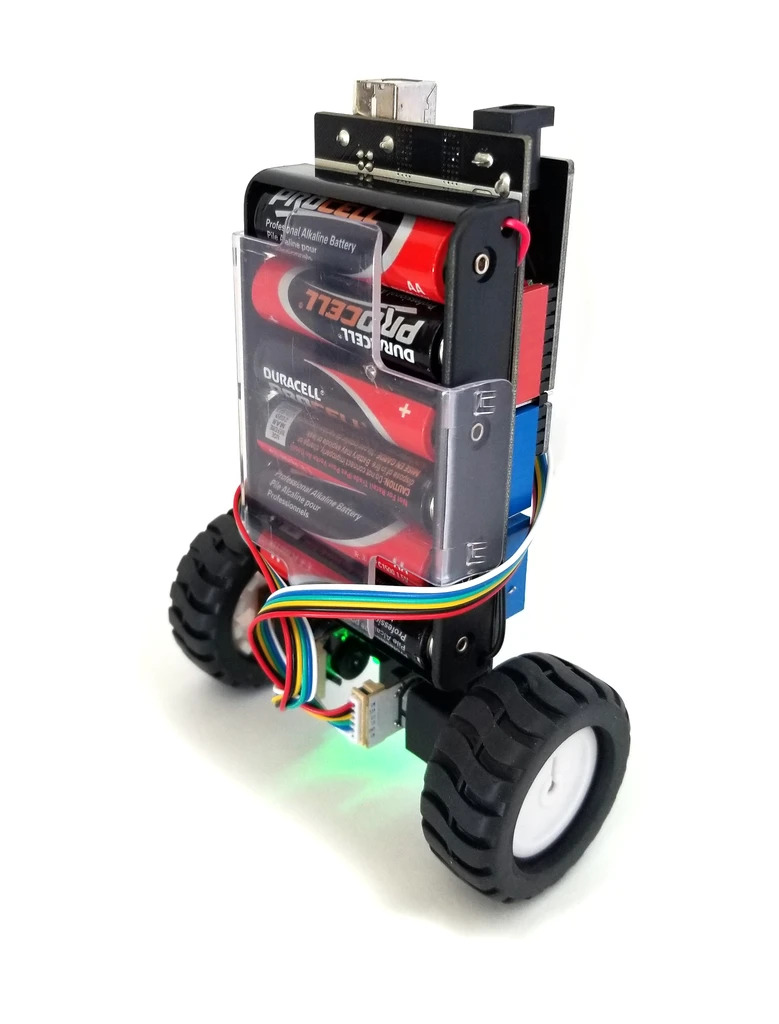
\includegraphics[height = 5.5cm]{minseg-M2V5}
	\end{center}
	\note<1-1>{\begin{itemize}
		\item maybe make Florian do some simple 'voice-music'
	\end{itemize}}
\end{frame}


\setbeamercolor{background canvas}{bg=white!80!black}
\begin{frame}{What are we doing today?}
	\begin{itemize}
		\item today we recap the P controller, and what it means
		\item we then add two more ingredients to our 'artificial brain' that we are putting into our robot: the I controller and D controller
		\item by mixing these three ingredients we will get our 'final' brain, a PID controller, a brain that is used practically everywhere, in the whole world
	\end{itemize}
\end{frame}
\setbeamercolor{background canvas}{bg=white}


\begin{frame}{Our purposes}
	\pause
	\begin{itemize}
		\item have fun
		\pause
		\item understand the world a bit better
		\pause
		\item see that math is useful
	\end{itemize}
\end{frame}


\begin{frame}{What is going to happen in today's part}
	\pause
	\begin{itemize}
		\item recall what is the ``P controller''
		\pause
		\item introduce the ``I and D controllers''
		\pause
		\item connect I and D with useful math concepts
	\end{itemize}
	\note<1-1>{\begin{itemize}
		\item we will see also how these controllers are naturally connected with two math concepts that a lot of students hate -- but they should not be hated! They are cute, simple and - most importantly - very useful!
	\end{itemize}}
\end{frame}


\setbeamercolor{background canvas}{bg=white!80!black}
\begin{frame}{Connecting things}
	\begin{itemize}
		\item let's recall what the P controller was, and how we arrived to it
	\end{itemize}
\end{frame}
\setbeamercolor{background canvas}{bg=white}


\begin{frame}{Towards the P controller: our first heuristic}
	\begin{center}
		\begin{tikzpicture}
			[
				body/.style = {rectangle, minimum width = 0.7cm, minimum height = 2.4cm, rounded corners, fill = black},
				wheel/.style = {circle, minimum size = 1.4cm, thick, fill = black!50!white, draw = black},
			]
			\node (body) [body, rotate = -30] {};
			\node (wheel) [wheel] at (body.south) {};
		\end{tikzpicture} \\
		$\implies$ spin the wheels as fast as possible clockwise
	\end{center}
	\note<1-1>{\begin{itemize}
		\item this approach is problematic because
		\item this controller is ``too nervous'': as soon as we are not perfectly aligned then it reacts as much as it can
		\item in practice with the problem of making the pen stand we saw that it does not make too much sense
		\item (maybe re-show the example)
	\end{itemize}}
\end{frame}


\begin{frame}{Towards the P controller: our second heuristic}
	\begin{center}
		\begin{tikzpicture}
			[
				body/.style = {rectangle, minimum width = 0.7cm, minimum height = 2.4cm, rounded corners, fill = black},
				wheel/.style = {circle, minimum size = 1.4cm, thick, fill = black!50!white, draw = black},
				myline/.style = {dashed, \StrongPrimary, thick},
			]
			\node (body) [body, rotate = -5] {};
			\node (wheel) [wheel] at (body.south) {};
			\draw [myline] (wheel) -- ++(0,3);
			\draw [myline] (wheel) -- ++(0.3,2.7);
			\draw [myline] (wheel) -- ++(0.6,2.3);
		\end{tikzpicture} \\
		$\implies$ depending on the zone, spin the wheels more or less fast
	\end{center}
	\note<1-1>{\begin{itemize}
		\item recall that also this approach was a bit problematic
		\item it is like having a car driver that turns the wheel in a clumsy way
	\end{itemize}}
\end{frame}


\begin{frame}{The P (i.e., proportional) controller}
	\begin{center}
		\begin{tikzpicture}
			[
				body/.style = {rectangle, minimum width = 0.7cm, minimum height = 2.4cm, rounded corners, fill = black},
				wheel/.style = {circle, minimum size = 1.4cm, thick, fill = black!50!white, draw = black},
				myline/.style = {dashed, \StrongPrimary, thick},
			]
			\node (body) [body, rotate = -5] {};
			\node (wheel) [wheel] at (body.south) {};
			\draw [myline] (wheel) -- ++(0,3);
		\end{tikzpicture} \\
		$\implies$ speed of the wheels = $P \cdot $ angular error
	\end{center}
	\note<1-1>{\begin{itemize}
		\item so we moved to the 'proportional' controller, our friend P controller
		\item depending on the error, we have a proportional action
	\end{itemize}}
\end{frame}


\begin{frame}{Remember: $P$ is a design choice!}
	\begin{itemize}
		\item $P$ small implies a 'gentle' control action
		\item $P$ big implies an 'aggressive' control action
	\end{itemize}
\end{frame}


\setbeamercolor{background canvas}{bg=white!80!black}
\begin{frame}
	\begin{footnotesize}
	\begin{itemize}
		\item but our brain is not complete if we make it only using the P ingredient
		\item let me show you what I mean using another example (also to show how ubiquitous control is)
		\item assume that I want to balance a ball on a board, and make the ball stay at the center of the board
		\item my control action, that is, what I can do, is to move the board in this way
		\item what is a P controller here? it is that depending on how far the ball is from the center, I tilt more or less
		\item now remember: I may be more or less aggressive, that means choosing P bigger or smaller
		\item but pretend to be in the open space now, and that there is some wind that is keeping blowing and pushing just a tiny bit the ball that I am balancing
		\item what happens? let's have some wind assistant here: wind assistant, may you disturb me a bit?
		\item so the wind pushes, and the P controller reacts
		\item the wind makes a force, and the P controller makes a force too
		\item whenever the two forces are equal, then we get an equilibrium
		\item but at the equilibrium the ball is not at the point where I would like it to be
		\item somehow the P controller by itself is not ``smart enough'' to realize that there is this disturbance, and eliminate it
		\item let's see this through an animation
	\end{itemize}
	\end{footnotesize}
\end{frame}
\setbeamercolor{background canvas}{bg=white}


\begin{frame}[t]{No wind = no problems}
	\begin{center}
		\begin{tikzpicture}
		[
			board/.style = {rectangle, rounded corners = 0.1cm, fill = white!50!gray, draw = white!50!gray, minimum width = 7cm, minimum height = 0.2cm},
			boardcenter/.style = {circle, fill = black, draw = black, inner sep = 0cm, minimum size = 0.15cm},
			ball/.style = {circle, minimum size = 1cm, draw = black, very thick},
		]
			%
			\node (board) [board] {};
			\node (boardcenter) [boardcenter] at (board.center) {};
			\node (ball) [ball, anchor = south] at (board.north) {};
			%
		\end{tikzpicture}
	\end{center}
\end{frame}


\begin{frame}[t]{Some wind = some problems}
	\begin{center}
		\begin{tikzpicture}
		[
			board/.style = {rectangle, rounded corners = 0.1cm, fill = white!50!gray, draw = white!50!gray, minimum width = 7cm, minimum height = 0.2cm},
			boardcenter/.style = {circle, fill = black, draw = black, inner sep = 0cm, minimum size = 0.15cm},
			ball/.style = {circle, minimum size = 1cm, draw = black, very thick},
			wind/.style = {very thick, densely dotted, blue},
		]
			%
			\node (board) [board, rotate = 10] {};
			\node (boardcenter) [boardcenter] at (board.center) {};
			\node (ball) [ball, anchor = south] at (board.25) {};
			%
			\node (auxA) [coordinate, xshift = -1.0cm] at (ball.west) {};
			\node (auxB) [coordinate, yshift =  0.2cm, xshift = -0.3cm] at (auxA) {};
			\node (auxC) [coordinate, yshift = -0.2cm, xshift = -0.2cm] at (auxA) {};
			%
			\draw [wind] (auxA) -- ++(-2cm,0);
			\draw [wind] (auxB) -- ++(-2cm,0);
			\draw [wind] (auxC) -- ++(-2cm,0);
			%
			\draw [wind] (auxA) arc (-90:90:0.1);
			\draw [wind] (auxA) arc (90:-90:0.1);
			\draw [wind] (auxB) arc (-90:90:0.1);
			\draw [wind] (auxC) arc (90:-90:0.1);
			%
		\end{tikzpicture}
	\end{center}
	\vspace{0.5cm} 
	\pause
	\begin{center}
		\begin{tikzpicture}
		[
			axes/.style = {thick, -latex},
			signal/.style = {thick, \StrongPrimary},
		]
			%
			\draw [axes] (0,0) -- (8,0) node [below, pos = 0.5] {time};
			\draw [axes] (0,0) -- (0,3) node [left, pos = 0.5] {error};
			%
			\foreach \t in {2,3,4,5,6}
			{
				\only<\t-\t>
				{
					\draw [signal] (0,1) -- (\t-1,1);
					\node at (4,2) {after \t\ seconds};
				}
			}
			%
		\end{tikzpicture}
	\end{center}
\end{frame}


\begin{frame}{Discussion time!}
	\begin{center}
		\begin{tikzpicture}
		[
			board/.style = {rectangle, rounded corners = 0.1cm, fill = white!50!gray, draw = white!50!gray, minimum width = 7cm, minimum height = 0.2cm},
			boardcenter/.style = {circle, fill = black, draw = black, inner sep = 0cm, minimum size = 0.15cm},
			ball/.style = {circle, minimum size = 1cm, draw = black, very thick},
			wind/.style = {very thick, densely dotted, blue},
		]
			%
			\node (board) [board, rotate = 10] {};
			\node (boardcenter) [boardcenter] at (board.center) {};
			\node (ball) [ball, anchor = south] at (board.25) {};
			%
			\node (auxA) [coordinate, xshift = -1.0cm] at (ball.west) {};
			\node (auxB) [coordinate, yshift =  0.2cm, xshift = -0.3cm] at (auxA) {};
			\node (auxC) [coordinate, yshift = -0.2cm, xshift = -0.2cm] at (auxA) {};
			%
			\draw [wind] (auxA) -- ++(-2cm,0);
			\draw [wind] (auxB) -- ++(-2cm,0);
			\draw [wind] (auxC) -- ++(-2cm,0);
			%
			\draw [wind] (auxA) arc (-90:90:0.1);
			\draw [wind] (auxA) arc (90:-90:0.1);
			\draw [wind] (auxB) arc (-90:90:0.1);
			\draw [wind] (auxC) arc (90:-90:0.1);
			%
		\end{tikzpicture}
	\end{center}
	\vspace{0.5cm} 
	\begin{center}
		\begin{tikzpicture}
		[
			axes/.style = {thick, -latex},
			signal/.style = {thick, \StrongPrimary},
		]
			%
			\draw [axes] (0,0) -- (8,0) node [below, pos = 0.5] {time};
			\draw [axes] (0,0) -- (0,3) node [left, pos = 0.5] {error};
			%
			\draw [signal] (0,1) -- (7,1);
			\node at (4,2) {\ItBoldPrimary{how may we solve this problem?}};
			%
		\end{tikzpicture}
	\end{center}
\end{frame}


\setbeamercolor{background canvas}{bg=white!80!black}
\begin{frame}
	\begin{itemize}
		\item got some intuition? shared it with your friends?
		\item let's see if we have the same idea!
		\item let's see if you discovered the I controller by yourself!
	\end{itemize}
\end{frame}
\setbeamercolor{background canvas}{bg=white}


\begin{frame}{The I (integral) ingredient: tilt not only proportionally to the current error, but also keep in mind the past history!}
	\vspace{0.2cm} 
	\begin{center}
		\begin{tikzpicture}
		[
			board/.style = {rectangle, rounded corners = 0.1cm, fill = white!50!gray, draw = white!50!gray, minimum width = 7cm, minimum height = 0.2cm},
			boardcenter/.style = {circle, fill = black, draw = black, inner sep = 0cm, minimum size = 0.15cm},
			ball/.style = {circle, minimum size = 1cm, draw = black, very thick},
			wind/.style = {very thick, densely dotted, blue},
		]
			%
			\node (board) [board, rotate = 10] {};
			\node (boardcenter) [boardcenter] at (board.center) {};
			\node (ball) [ball, anchor = south] at (board.25) {};
			%
			\node (auxA) [coordinate, xshift = -1.0cm] at (ball.west) {};
			\node (auxB) [coordinate, yshift =  0.2cm, xshift = -0.3cm] at (auxA) {};
			\node (auxC) [coordinate, yshift = -0.2cm, xshift = -0.2cm] at (auxA) {};
			%
			\draw [wind] (auxA) -- ++(-2cm,0);
			\draw [wind] (auxB) -- ++(-2cm,0);
			\draw [wind] (auxC) -- ++(-2cm,0);
			%
			\draw [wind] (auxA) arc (-90:90:0.1);
			\draw [wind] (auxA) arc (90:-90:0.1);
			\draw [wind] (auxB) arc (-90:90:0.1);
			\draw [wind] (auxC) arc (90:-90:0.1);
			%
		\end{tikzpicture}
	\end{center}
	\vspace{0.1cm} 
	\begin{center}
		\begin{tikzpicture}
		[
			axes/.style = {thick, -latex},
			signal/.style = {thick, \StrongPrimary},
		]
			%
			\draw [axes] (0,0) -- (8,0) node [below, pos = 0.5] {time};
			\draw [axes] (0,0) -- (0,3) node [left, pos = 0.5] {error};
			%
			\draw [signal] (0,1) -- (7,1);
			\node at (6,2.5) {P ingredient = ``how much error do we have now''};
			\node at (6,1.5) {I ingredient = ``how much error have we accumulated''};
			%
		\end{tikzpicture}
	\end{center}
	\note<1-1>{\begin{itemize}
		\item here I would explain things graphically with the graphical tablet
		\item make clear that $I$ is a design choice
	\end{itemize}}
\end{frame}


\setbeamercolor{background canvas}{bg=white!80!black}
\begin{frame}
	\begin{itemize}
		\item but, as before, how do we design $I$?
		\item to understand we should ask ourselves: what is the effect of having different $I$s?
		\item if I put $I = $ a tiny tiny number, what is going to happen?
		\item if I put $I = $ a huge number, what is going to happen?
		\item let's have a chat all together, and see what we think about this
	\end{itemize}
\end{frame}
\setbeamercolor{background canvas}{bg=white}


\begin{frame}{Discussion time!}
	\begin{itemize}
		\item if I put $I = $ a tiny tiny number, what is going to happen?
		\item if I put $I = $ a huge number, what is going to happen?
	\end{itemize}
\end{frame}


\setbeamercolor{background canvas}{bg=white!80!black}
\begin{frame}
	\begin{itemize}
		\item good! So, the effects of choosing $I$ are kind of similar as before for $P$, but not quite the same: the bigger $I$, the more we use the past to decide what to do now
		\item uhm, using the past errors to decide what to do now\ldots and may we also use the future errors to decide what to do now? Can we forecast which errors we are going to make in the future?
	\end{itemize}
\end{frame}
\setbeamercolor{background canvas}{bg=white}


\setbeamercolor{background canvas}{bg=white!80!red}
\begin{frame}
	\begin{itemize}
		\item (this may be too much) 4 seconds of Sofie dressed like a magician making faces like she is trying to predict the future
	\end{itemize}
\end{frame}
\setbeamercolor{background canvas}{bg=white}


\begin{frame}{Predicting the future errors}
	\begin{center}
		\begin{tikzpicture}
		\begin{axis}
		[
			xmode					= linear,
			ymode					= linear,
			width					= 0.8\columnwidth,
			height					= 0.45\columnwidth,
			axis x line				= bottom,	% bottom | middle | top
			axis y line				= left,		% left | middle | right
			xtick					= {0,...,4},
			ytick					= {0,...,4},
			xmin					= 0,
			xmax					= 5,
			ymin					= 0,
			ymax					= 5,
			xlabel					= {time},
			ylabel					= {error},
		]
			%
			\addplot
			[
				no marks,
				smooth,
				domain	= 0:3,
				samples = 100,
			]
			{(x^2 + 3)/(x + 1)};
			%
		\end{axis}
		\end{tikzpicture}
	\end{center}
	\note<1-1>{\begin{itemize}
		\item easiest way of predicting = prolong given the current slope
		\item slope = derivative
	\end{itemize}}
\end{frame}


\begin{frame}{The D (derivative) ingredient: tilt not only proportionally to the current error and keeping in mind the past history, but also forecasting what is going to happen in the future!}
	\pause
	$$
		\text{my action} = 
		\pause
			P \cdot \text{current error}
		\pause
		+	I \cdot \text{area of past error}
		\pause
		+	D \cdot \text{slope of current error}
	$$
	\note<1->{\begin{itemize}
		\item the overall action combines all the single actions
		\item the brain that we put in the robot is composed by 3 parts that help each other, and have kind of different purposes
	\end{itemize}}
\end{frame}


\setbeamercolor{background canvas}{bg=white!80!black}
\begin{frame}
	\begin{itemize}
		\item let's make a summary:
		\item P is how much I react to the current error
		\item I is a memory term: if I have been making errors for some time, then compensate for them
		\item D is trying to compensate for what I think the error will be in the next future. But watch out, predicting the future is a challenging thing, and the D term may make your brain quite nervous; try later on to put D big and you will see
	\end{itemize}
\end{frame}
\setbeamercolor{background canvas}{bg=white}


\begin{frame}{I and D, two concepts that you will encounter in the future!}
	\begin{itemize}
		\item I = integral = area; symbol:
			$$
				\int e(t) dt
			$$
		\item D = derivative = slope; symbol
			$$
				\frac{d e(t)}{d t}
			$$
	\end{itemize}
	\note<1-1>{\begin{itemize}
		\item maybe say that ``they are actually one the inverse of the other one, but no worries - you will have time to understand why''
	\end{itemize}}
\end{frame}


\setbeamercolor{background canvas}{bg=white!80!black}
\begin{frame}
	\begin{itemize}
		\item and now I leave you with playing with the robot; choose different $P$s, different $I$s, and different $D$s, and see what happens
		\item my proposal: make a robot race! let's see who finds the best combination!
	\end{itemize}
\end{frame}
\setbeamercolor{background canvas}{bg=white}


\begin{frame}
	\begin{center}
		$\rightarrow$ ``manual for the students'', section ``experimenting with the PID controller''
	\end{center}
	\note<1-1>{\begin{itemize}
		\item for this, go to the manual and follow the instructions reported there in this section
	\end{itemize}}
\end{frame}


\setbeamercolor{background canvas}{bg=white!80!black}
\begin{frame}
	\begin{itemize}
		\item so, now I let you do, and close this series video - I hope you liked it and that in the why you learned something about the most common automatic control strategy, the PID controller!
		\item please feel free to keep in touch, and good luck with all your wonderful projects!
		\item bye!
	\end{itemize}
\end{frame}
\setbeamercolor{background canvas}{bg=white}


\title	[Balancing Robots]	{Making robots balance}
\begin{frame}
	\titlepage
	\vspace{-2.5cm} 
	\begin{center}
	 	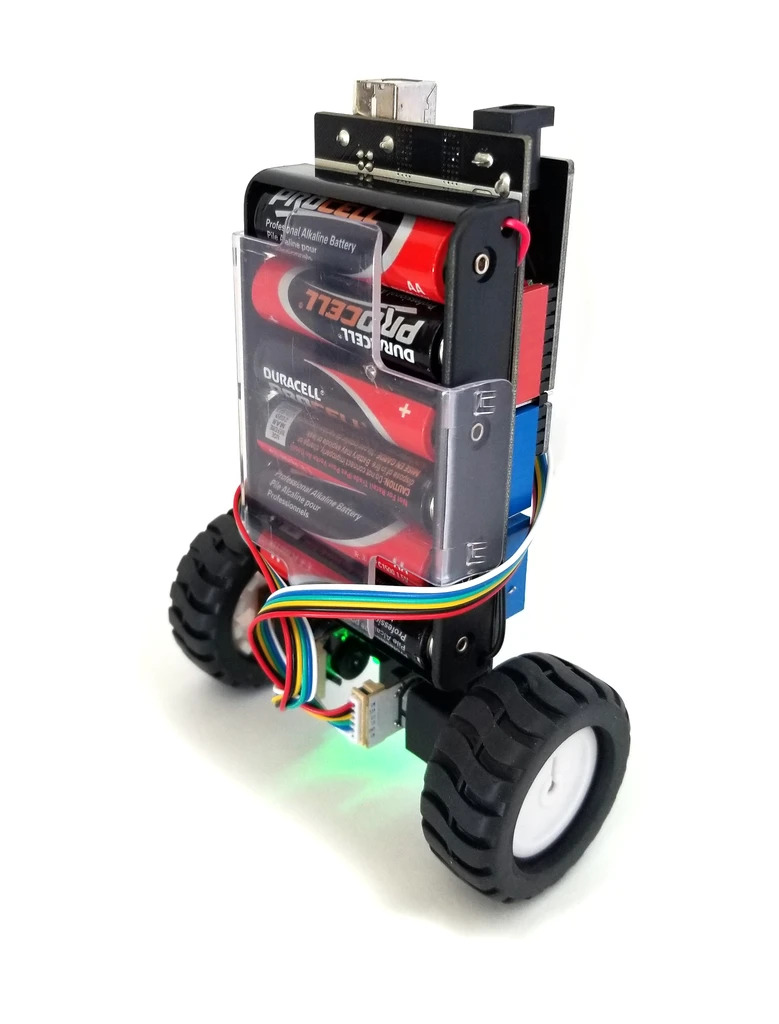
\includegraphics[height = 5.5cm]{minseg-M2V5} \\
		\texttt{steffi.knorn@ovgu.de}
	\end{center}
\end{frame}


\setbeamercolor{background canvas}{bg=white!80!red}
\begin{frame}
	\begin{itemize}
		\item any Easter egg you would like to add :)
	\end{itemize}
\end{frame}
\setbeamercolor{background canvas}{bg=white}



% ~~~~~~~~~~~~~~~~~~~~~~~~~~~~~~~~~~~~~~~~~~~~~~~~~~~~~~~~~~~~~~~~~ %
\end{document}														%
% ~~~~~~~~~~~~~~~~~~~~~~~~~~~~~~~~~~~~~~~~~~~~~~~~~~~~~~~~~~~~~~~~~ %
% ./FramesTemplates/template__citation.tex
% ./FramesTemplates/template__empty_frame.tex
% ./FramesTemplates/template__frame_with_blocks.tex
% ./FramesTemplates/template__frame_with_colored_background.tex
% ./FramesTemplates/template__frame_with_itemized_list.tex
% ./FramesTemplates/template__frame_with_overlayed_figures.tex
% ./FramesTemplates/template__frame_with_two_columns.tex
% ./FramesTemplates/template__frame_with_two_columns_and_overlayed_figures.tex


\begin{frame}{<++>}{<++>}
	<++>
	\note<1-1>{\begin{itemize}
		\item <++>
	\end{itemize}}
\end{frame}
<++>


